\chapter*{Введение} % * не проставляет номер
\addcontentsline{toc}{chapter}{Введение} % вносим в содержание

Двухтональный многочастотный набор (DTMF) — это метод представления цифр клавиатуры телефона тонами для передачи по аналоговому каналу связи. Технология DTMF представляет собой надежную альтернативу роторным телефонным системам и позволяет пользователю вводить данные во время телефонного разговора (\firef{fig:dtmf}). Эта функция позволила создать интерактивные системы автоматического ответа, такие как системы, используемые для телефонного банкинга, маршрутизации звонков в службу поддержки клиентов, голосовой почты и других подобных приложений.

\begin{figure}[ht] 
	\center
	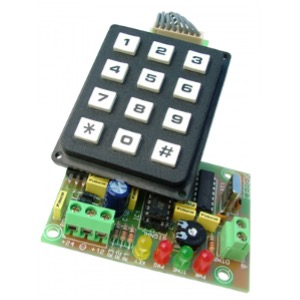
\includegraphics [scale=0.7] {my_folder/images/dtmf}
	\caption{Физическое устройство для работы с DTMF-сигналами} 
	\label{fig:dtmf}
	\end{figure}

Для кодирования символа в DTMF сигнал необходимо сложить два синусоидальных сигнала. Частоты синусоид берутся по приведённой ниже \taref{tab:lrt} из столбца и строки, соответствующих передаваемому символу. Каждая строка набора представлена частотой низкого тона, а каждый столбец - частотой высокого тона.

\begin{table}[ht]
\centering\small
	\caption{Таблица соответствия частот и символов DTMF}
	\label{tab:lrt}	
\begin{tabular}{|c|c|c|c|l|}
\hline
\multicolumn{1}{|l|}{\textbf{1209 Гц}} & \multicolumn{1}{l|}{\textbf{1336 Гц}} & \multicolumn{1}{l|}{\textbf{1477 Гц}} & \multicolumn{1}{l|}{\textbf{1633 Гц}} &                 \\ \hline
1                                      & 2                                     & 3                                     & A                                     & \textbf{697 Гц} \\ \hline
4                                      & 5                                     & 6                                     & B                                     & \textbf{770 Гц} \\ \hline
7                                      & 8                                     & 9                                     & C                                     & \textbf{852 Гц} \\ \hline
*                                      & 0                                     & \#                                    & D                                     & \textbf{941 Гц} \\ \hline
\end{tabular}\normalsize% возвращаем шрифт к нормальному
\end{table}

Частоты, выбранные для тонов DTMF, имеют некоторые отличительные характеристики и уникальные свойства:

\begin{itemize}
	\item все тона находятся в слышимом диапазоне частот, что позволяет человеку определить, когда была нажата клавиша;
	\item ни одна частота не является кратной другой;
	\item сумма или разность любых двух частот не равна другой выбранной частоте.
\end{itemize} 

Второе и третье свойства упрощают декодирование DTMF и уменьшают количество ложно распознанных тонов. Уникальные свойства позволяют приемникам DTMF определять, когда пользователь нажимает несколько клавиш одновременно.

Цель данной работы заключается в создании инструмента для генерации DTMF-сигналов и распознавания их в звуковом файле соответственно.

Для достижения поставленной цели необходимо выполнить следующие задачи:

\begin{itemize}
	\item изучить теоретических материалов по моделированию DTMF-сигналов;
	\item реализовать метод генерации двухтонального многочастотного сигнала;
	\item изучить материалы по распознаванию DTMF-сигналов;
	\item выбрать и реализовать одним из методов декодирования.
\end{itemize} 

В результате данной работы предполагается создание программного инструмента, который способен как моделировать DTMF-сигналы из входящего набора символов, так и декодировать звуковую дорожку в сообщение. 

%% Вспомогательные команды - Additional commands
%\newpage % принудительное начало с новой страницы, использовать только в конце раздела
%\clearpage % осуществляется пакетом <<placeins>> в пределах секций
%\newpage\leavevmode\thispagestyle{empty}\newpage % 100 % начало новой строки